\documentclass[12pt,a4paper]{article}
\usepackage[utf8]{inputenc} % inutile avec XeLaTeX/LuaLaTeX
\usepackage[T1]{fontenc}
\usepackage{amsmath,amssymb,mathrsfs,tikz,times,pifont}
\usepackage{enumitem}
\usepackage{multicol}
\usepackage{lmodern}
\newcommand\circitem[1]{%
\tikz[baseline=(char.base)]{
\node[circle,draw=gray, fill=red!55,
minimum size=1.2em,inner sep=0] (char) {#1};}}
\newcommand\boxitem[1]{%
\tikz[baseline=(char.base)]{
\node[fill=cyan,
minimum size=1.2em,inner sep=0] (char) {#1};}}
\setlist[enumerate,1]{label=\protect\circitem{\arabic*}}
\setlist[enumerate,2]{label=\protect\boxitem{\alph*}}
\everymath{\displaystyle}
\usepackage[left=1cm,right=1cm,top=1cm,bottom=1.7cm]{geometry}
\usepackage[colorlinks=true, linkcolor=blue, urlcolor=blue, citecolor=blue]{hyperref}
\usepackage{array,multirow}
\usepackage[most]{tcolorbox}
\usepackage{varwidth}
\usepackage{float}
\tcbuselibrary{skins,hooks}
\usetikzlibrary{patterns}
\usepackage{tikz}
\usetikzlibrary{arrows, shapes.geometric, fit}

\usepackage{pgfplots}
\pgfplotsset{compat=1.18}
\newtcolorbox{exa}[2][]{enhanced,breakable,before skip=2mm,after skip=5mm,
colback=yellow!20!white,colframe=black!20!blue,boxrule=0.5mm,
attach boxed title to top left ={xshift=0.6cm,yshift*=1mm-\tcboxedtitleheight},
fonttitle=\bfseries,
title={#2},#1,
boxed title style={frame code={
\path[fill=tcbcolback!30!black]
([yshift=-1mm,xshift=-1mm]frame.north west)
arc[start angle=0,end angle=180,radius=1mm]
([yshift=-1mm,xshift=1mm]frame.north east)
arc[start angle=180,end angle=0,radius=1mm];
\path[left color=tcbcolback!60!black,right color = tcbcolback!60!black,
middle color = tcbcolback!80!black]
([xshift=-2mm]frame.north west) -- ([xshift=2mm]frame.north east)
[rounded corners=1mm]-- ([xshift=1mm,yshift=-1mm]frame.north east)
-- (frame.south east) -- (frame.south west)
-- ([xshift=-1mm,yshift=-1mm]frame.north west)
[sharp corners]-- cycle;
},interior engine=empty,
},interior style={top color=yellow!5}}

\usepackage{fancyhdr}
\usepackage{eso-pic}
\usepackage{tkz-tab}
\AddToShipoutPicture{
    \AtTextCenter{%
        \makebox[0pt]{\rotatebox{80}{\textcolor[gray]{0.7}{\fontsize{5cm}{5cm}\selectfont PGB}}}
    }
}

\usepackage{verbatim}

\usepackage{color,soul}

\newenvironment{remarque}{\smallskip\noindent\textbf{Remarque : }\itshape}{\smallskip}

\usepackage{amsmath}
\usepackage{amsfonts}
\usepackage{amssymb}
\usepackage{systeme}
\usepackage{tkz-tab}
\usepackage{tikz}
\usetikzlibrary{arrows}
\newcounter{exemple} % Compteur pour les questions

% Définir la commande pour afficher une question numérotée
\newcommand{\exemple}{%
  \refstepcounter{exemple}%
  \textbf{\textcolor{green}{Exemple \theexemple :}} \ignorespaces
}
%---------------------------------------
\definecolor{myorange}{rgb}{1.0, 0.8, 0.0}

% Définir un compteur pour les exercices d'application
\newcounter{exerciceapp}

% Définir la commande pour afficher un exercice d'application numéroté
\newcommand{\exerciceapp}{%
  \refstepcounter{exerciceapp}%
  \textbf{\textcolor{myorange}{Exercice d'application \theexerciceapp :}} \ignorespaces
}
%--------------------------------------
% Définir un compteur pour les exercices d'application
\newcounter{correction}

% Définir la commande pour afficher un correction exercice d'application numéroté
\newcommand{\correction}{%
  \refstepcounter{correction}%
  \textbf{\textcolor{myorange}{Correction \thecorrection :}} \ignorespaces
}
%--------------------------------------
% Commande pour ajouter du texte en arrière-plan
\usepackage{fancyhdr}
\usepackage{eso-pic}
%\usepackage{tkz-tab}
\AddToShipoutPicture{
    \AtTextCenter{%
        \makebox[0pt]{\rotatebox{80}{\textcolor[gray]{0.7}{\fontsize{5cm}{5cm}\selectfont PGB}}}
    }
}
%This command takes a colour as an optional argument; the default colour is black.
\usetikzlibrary{shapes.geometric,fit}
\newcommand{\myul}[2][black]{\setulcolor{#1}\ul{#2}\setulcolor{black}}
\newcommand\tab[1][1cm]{\hspace*{#1}}

\begin{document}
% En-tête personnalisée
\begin{center}
    \Large\textbf{\underline{\textcolor{red}{Équation Différentielle (\(\neq\))}}}\\[-0.1cm]
    \normalsize\textbf{Prof : M. BA} \hfill \textbf{Classe : TS2}\\[-0.1cm]
    \textbf{Année scolaire : 2025 -- 2026}
\end{center}

\section*{\underline{\textbf{\textcolor{red}{I. Définitions}}}}
Soient $a_{0},a_{1},...,a_{n}$ des constantes réelles, $y=y(x)$ une fonction de 
$x$. On appelle \textbf{équation différentielle linéaire d'ordre $n$ à coefficients constants}, une équation liant une fonction $y$ et ses dérivées successives $y',y'',\cdots , y^{n}$. On a $a_{n}y^{n}(x)+a_{n-1}y^{n-1}(x)+\cdots +a_{2}y''(x)+a_{1}y'(x)+a_{0}y(x)=g(x)$ où $g(x)$ est une fonction donnée appelée second membre et $a_{n}\neq 0$

\subsection*{\underline{\textbf{\textcolor{red}{Exemple}}}}
L'équation $2y'' - 3y' + 4y = \sin(2x)$ est une équation différentielle linéaire du 2\textsuperscript{nd} ordre, à coefficients constants.

\begin{itemize}
    \item L'équation \textbf{(E)} : $a_{n}y^{(n)} + a_{n-1}y^{(n-1)} + \dots + a_{1}y' + a_{0}y = g(x)$ est dite  \textbf{équation avec second membre}. 
    
    \item L'équation \textbf{(E')} : $a_{n}y^{(n)} + a_{n-1}y^{(n-1)} + \dots + a_{1}y' + a_{0}y = 0$ est dite \textbf{équation homogène} ou \textbf{équation sans second membre}. 	   
    
    \item \textbf{(E')} est appelée l'équation homogène \textbf{associée} à \textbf{(E)}.
    
    \item Les solutions d'une équation différentielle sont des \textbf{fonctions}.
    
    \item Une fonction $f$ est solution de l'équation différentielle sur un intervalle $I$ si elle est $n$ fois dérivable sur $I$ et si elle vérifie l'équation pour tout $x \in I$.
    
    \item L'ensemble de toutes les solutions d'une équation différentielle est appelé la \textbf{solution générale} de l'équation.
    
    \item Toute fonction particulière qui vérifie l'équation différentielle est appelée une \textbf{solution particulière}.
\end{itemize}

\section*{\underline{\textbf{\textcolor{red}{II. Théorèmes de superposition}}}}

Soient $(E)$ une équation différentielle linéaire d'ordre $n$ à coefficients constants avec second membre, et $(E')$ l'équation homogène associée.

\subsection*{\underline{\textbf{\textcolor{red}{Propriété 1 : Cas de l'équation homogène}}}}
Si $y_1$ et $y_2$ sont deux solutions de l'équation homogène $(E')$, alors leur somme $y_1 + y_2$ est encore une solution de $(E')$.

\begin{remarque}
Plus généralement, toute combinaison linéaire $\lambda y_1 + \mu y_2$ (où $\lambda, \mu \in \mathbb{R}$) est aussi solution de $(E')$.
\end{remarque}

\subsection*{\underline{\textbf{\textcolor{red}{Propriété 2 : Cas de l'équation complète}}}}
Si $y_h$ est une solution de l'équation homogène $(E')$ et $y_p$ est une solution de l'équation avec second membre $(E)$, alors leur somme :
$ y(x) = y_h(x) + y_p(x)$
est encore une solution de l'équation complète $(E)$.

\begin{comment}
-------------------------------------------------------

\section*{\underline{\textbf{\textcolor{red}{Démonstrations des théorèmes de superposition}}}}

Pour simplifier l'écriture, on note $L(y)$ l'expression du premier membre de l'équation :
\[ L(y) = a_{n}y^{(n)} + a_{n-1}y^{(n-1)} + \dots + a_{1}y' + a_{0}y \]
Ainsi, l'équation complète s'écrit $L(y) = g(x)$ et l'équation homogène s'écrit $L(y) = 0$.

Grâce aux propriétés de la dérivation, pour toutes fonctions $u$ et $v$ dérivables $n$ fois, on a :
\[ (u+v)' = u' + v', \quad (u+v)'' = u'' + v'', \quad \dots \quad (u+v)^{(n)} = u^{(n)} + v^{(n)} \]
On en déduit la propriété de linéarité essentielle : $L(u + v) = L(u) + L(v)$.

\subsection*{\underline{\textbf{\textcolor{red}{Preuve de la Propriété 1 (Cas homogène)}}}}

\textbf{Hypothèses :} $y_1$ et $y_2$ sont deux solutions de $(E')$, ce qui signifie que :
\[ L(y_1) = 0 \quad \text{et} \quad L(y_2) = 0 \]

\textbf{Calcul :} Utilisons la propriété de linéarité pour la fonction somme $(y_1 + y_2)$ :
\[ L(y_1 + y_2) = L(y_1) + L(y_2) \]
En remplaçant par les hypothèses, on obtient :
\[ L(y_1 + y_2) = 0 + 0 = 0 \]

\textbf{Conclusion :} L'expression s'annule, donc la fonction $y_1 + y_2$ est bien solution de l'équation homogène $(E')$.

\subsection*{\underline{\textbf{\textcolor{red}{Preuve de la Propriété 2 (Cas complet)}}}}

\textbf{Hypothèses :} $y_h$ est solution de $(E')$ et $y_p$ est solution de $(E)$, ce qui signifie que :
\[ L(y_h) = 0 \quad \text{et} \quad L(y_p) = g(x) \]

\textbf{Calcul :} Posons la fonction somme $y = y_h + y_p$ et injectons-la dans l'opérateur $L$ :
\[ L(y) = L(y_h + y_p) \]
Par linéarité, on sépare les termes :
\[ L(y) = L(y_h) + L(y_p) \]
En remplaçant par les valeurs de nos hypothèses :
\[ L(y) = 0 + g(x) = g(x) \]

\textbf{Conclusion :} On obtient exactement $L(y) = g(x)$, ce qui prouve que la fonction $y = y_h + y_p$ est bien solution de l'équation complète $(E)$.

++++++++++++++++++++++++++++++++++++++++++++++++++++++
\end{comment}

\subsection*{\underline{\textbf{\textcolor{green}{Preuve[Propriété 1]}}}}
\textbf{A faire}
\subsection*{\underline{\textbf{\textcolor{green}{Preuve[Propriété 2]}}}}
Soit $f_p$ une solution particulière de l'équation \textbf{(E)} avec second membre, et $f_h$ une solution générale de l'équation homogène associée \textbf{(E')}. Nous devons montrer que $f(x) = f_p(x) + f_h(x) $ est une solution générale de l'équation \textbf{(E)}.

Puisque $f_p$ est une solution particulière de \textbf{(E)}, cela signifie que lorsque nous remplaçons $y$ par $f_p$ dans \textbf{(E)}, nous obtenons une équation vraie. 

C'est-à-dire : \textcolor{green}{$ a_{n}f_p^{(n)}(x) + a_{n-1}f_p^{(n-1)}(x) + \ldots + a_{2}f_{p}''(x) + a_{1}f_{p}'(x) + a_{0}f_{p}(x)=g(x) $}

De même, puisque $f_h$ est une solution générale de \textbf{(E')}, lorsque nous remplaçons $y$ par $f_h$ dans \textbf{(E')}, nous obtenons une équation vraie.

C'est-à-dire : \textcolor{blue}{$ a_{n}f_{h}^{(n)}(x)+a_{n-1}f_{h}^{(n-1)}(x)+\cdots+a_{2}f_{h}^{''}(x)+a_{1}f_{h}^{'}(x)+a_{0}f_{h}(x)=0 $}

En ajoutant les deux équations, nous obtenons l'équation :

$\textcolor{green}{a_{n}f_p^{(n)}(x) + a_{n-1}f_p^{(n-1)}(x) + \ldots + a_{2}f_{p}''(x) + a_{1}f_{p}'(x) + a_{0}f_{p}(x)}$ + $\textcolor{blue}{a_{n}f_h^{(n)}(x) + a_{n-1}f_h^{(n-1)}(x) +}$ 
\[\textcolor{blue}{\ldots + a_{2}f_{h}''(x) + a_{1}f_{h}'(x) + a_{0}f_{h}(x)}\]
\[=\textcolor{green}{g(x)}+\textcolor{blue}{0}\]

\[a_{n}(f_{p}+f_{h})^{(n)}(x)+a_{n-1}(f_{p}+f_{h})^{(n-1)}(x)+\cdots+a_{2}(f_{p}+f_{h})^{''}(x)+a_{1}(f_{p}+f_{h})'(x)+a_{0}(f_{p}+f_{h})(x)=g(x)\]
Puisque $f_p$ est une solution de l'équation avec second membre \textbf{(E)} et $f_h$ est une solution de l'équation homogène \textbf{(E')}, la partie gauche de l'équation ci-dessus est égale à $g(x) + 0$, ce qui est simplement $g(x)$. Ainsi,\\ $f(x) = f_p(x) + f_h(x)$ satisfait l'équation différentielle \textbf{(E)}, ce qui prouve que c'est une solution générale de \textbf{(E)}.

\section*{\underline{\textbf{\textcolor{red}{
\begin{minipage}[t]{\textwidth}III. Équations différentielles linéaires d'ordre 1, à coefficients constants
\end{minipage}}}}}
Une équation différentielle linéaire d'ordre 1, à coefficients constants est une équation de la forme
 \[\textbf{(E)}: ay'+by=g(x)\textbf{(avec second membre)} \]
 \[\textbf{(E')}: ay'+by=0\textbf{(sans second membre ou équation homogène)}\]
\subsection*{\underline{\textbf{\textcolor{red}{1. Recherche de la solution générale de l'équation homogène}}}}
$
\begin{aligned}
\textbf{Soit } \textbf{(E')} : ay'+by=0 \textbf{ où a et b sont des réels avec a } \neq 0 \textbf{  alors, } ay'=-by &\Longrightarrow \frac{y'}{y}=-\frac{b}{a}\\
                                                                 &\Longrightarrow \ln|y|=-\frac{b}{a}x+c\\
                                                                 &\Longrightarrow |y|=e^{-\frac{b}{a}x+c}\\
                                                                 &\Longrightarrow |y|=e^{c}.e^{-\frac{b}{a}x}\\
                                                                 &\Longrightarrow y=\pm e^{c}.e^{-\frac{b}{a}x}\end{aligned}
$

En posant $k = \pm e^c$, on obtient $y = k e^{-\frac{b}{a}x}$ avec $k \in \mathbb{R}^*$. 

\begin{remarque}
La fonction nulle ($y = 0$, qui correspond au cas $k = 0$) est également une solution évidente de l'équation $(E')$. On peut donc étendre la constante $k$ à toutes les valeurs réelles.
\end{remarque}


\textbf{Conclusion :} Les solutions générales de l'équation homogène $(E')$ sont les fonctions $f_h$ (ou $y_h$) définies sur $\mathbb{R}$ de la forme :
$ f_h(x) = k e^{-\frac{b}{a}x} \quad \text{où } k \in \mathbb{R} $

\noindent\textbf{Exemple :} 
Résoudre sur $\mathbb{R}$ l'équation différentielle homogène $(E_1) : 2y' + 3y = 0$.

\textbf{Solution :} 
Ici, $a = 2$ et $b = 3$. D'après le cours, les solutions générales de cette équation sont les fonctions $y_h$ définies sur $\mathbb{R}$ par :
$ y_h(x) = k e^{-\frac{3}{2}x} \quad \text{où } k \in \mathbb{R} $
\subsection*{\underline{\textbf{\textcolor{red}{2. Recherche d'une solution particulière de l'équation avec second membre}}}}

Soit l'équation différentielle complète (avec second membre) $(E) : ay'(x) + by(x) = g(x)$.

\begin{itemize}
    \item Une fonction $y_p$ est dite \textbf{solution particulière} de $(E)$ si elle est dérivable sur $\mathbb{R}$ et si elle vérifie l'équation complète : 
    $ a y_p'(x) + b y_p(x) = g(x) $
    
    \item \textbf{Cas où $g(x)$ est un polynôme :} Si $g(x)$ est un polynôme de degré $n$ et que $b \neq 0$, alors on cherche la solution particulière $y_p$ sous la forme d'un polynôme de même degré $n$.
    
    \item \textbf{Cas où $g(x)$ est de forme trigonométrique :} Si $g(x)$ est de la forme $\alpha \cos(\beta x) + \mu \sin(\beta x)$ (où $\alpha$ et $\mu$ sont des constantes réelles), alors on cherche $y_p$ sous la forme :
    $ y_p(x) = A \cos(\beta x) + B \sin(\beta x) $
    où $A$ et $B$ sont deux constantes réelles à déterminer en injectant $y_p$ dans $(E)$.
\end{itemize}

\subsection*{\underline{\textbf{\textcolor{red}{Exemple :}}}}

\begin{itemize}

    \item 
    \noindent\textbf{Exemple :} 
    Trouver une solution particulière de l'équation $(E_2) : y' - 2y = 4x^2 - 2x$.
    
    \textbf{Solution :} 
    Le second membre $g(x) = 4x^2 - 2x$ est un polynôme de degré 2 et le coefficient devant $y$ est non nul ($b = -2 \neq 0$). On cherche donc $y_p$ sous la forme d'un polynôme de degré 2 : 
    \[ y_p(x) = Ax^2 + Bx + C \quad \Longrightarrow \quad y_p'(x) = 2Ax + B \]
    En injectant $y_p$ et $y_p'$ dans l'équation $(E_2)$, on obtient :
    \[ (2Ax + B) - 2(Ax^2 + Bx + C) = 4x^2 - 2x \quad \Longrightarrow \quad -2Ax^2 + (2A - 2B)x + (B - 2C) = 4x^2 - 2x \]
    
    \[\text{Par identification des coefficients, on résout le système :}
    \begin{cases}
    -2A = 4 \\
    2A - 2B = -2 \\
    B - 2C = 0
    \end{cases}
    \Longrightarrow
    \begin{cases}
    A = -2 \\
    B = -1 \\
    C = -\frac{1}{2}
    \end{cases}
    \]
    Ainsi, la solution particulière est : $y_p(x) = -2x^2 - x - \frac{1}{2}$.
    
    \textbf{Cas où $g(x)$ est de forme trigonométrique :} Si $g(x)$ est de la forme $\alpha \cos(\beta x) + \mu \sin(\beta x)$ (où $\alpha$ et $\mu$ sont des constantes réelles), alors on cherche $y_p$ sous la forme :
    $ y_p(x) = A \cos(\beta x) + B \sin(\beta x) $
    
    où $A$ et $B$ sont deux constantes réelles à déterminer en injectant $y_p$ dans $(E)$.
    
    \item 
    \noindent\textbf{Exemple :} 
    Trouver une solution particulière de l'équation $(E_3) : y' + y = 10\cos(2x)$.
    
    \textbf{Solution :} 
    Ici, $\beta = 2$. On cherche donc $y_p$ sous la forme :
    \[ y_p(x) = A \cos(2x) + B \sin(2x) \quad \Longrightarrow \quad y_p'(x) = -2A \sin(2x) + 2B \cos(2x) \]
    En injectant dans $(E_3)$, on a :
    $ (-2A \sin(2x) + 2B \cos(2x)) + (A \cos(2x) + B \sin(2x)) = 10\cos(2x) $
    
    En regroupant les termes en $\cos(2x)$ et $\sin(2x)$ :
    $ (A + 2B)\cos(2x) + (-2A + B)\sin(2x) = 10\cos(2x) $
    
    
    \[\text{Par identification, on obtient le système :}
    \begin{cases}
    A + 2B = 10 \\
    -2A + B = 0 
    \end{cases}
    \Longrightarrow
    \begin{cases}
     A = 2 \\
    B = 4
    \end{cases}
    \]
    La solution particulière est donc : $y_p(x) = 2\cos(2x) + 4\sin(2x)$.
\end{itemize}

\subsection*{\underline{\textbf{\textcolor{red}{3. Solution générale de \textbf{(E)}}}}}
Une solution générale $y(x)$ de l'équation complète \textbf{(E)} est donnée par :
$ y(x) = y_h(x) + y_p(x) $

où $y_h$ est la solution générale de l'équation homogène \textbf{(E')} et $y_p$ est une solution particulière de \textbf{(E)}.

\noindent\textbf{Exemple :} 
Résoudre sur $\mathbb{R}$ l'équation différentielle complète $(E_4) : y' + y = 10\cos(2x)$.

\textbf{Solution :}  
La solution générale de l'équation $(E_4)$ est la somme de ces deux fonctions. Les solutions sont donc les fonctions $y$ définies sur $\mathbb{R}$ par :
$ y(x) = y_h(x) + y_p(x) = k e^{-x} + 2\cos(2x) + 4\sin(2x) \quad \text{où } k \in \mathbb{R} $

\begin{comment}

\subsection*{\underline{\textbf{\textcolor{red}{Exercice d'application}}}}
Soit $\phi$ la fonction dérivable sur $\mathbb{R}$ solution de l'équation différentielle\\
\textbf{(E)}:$2y'-3y=x^{2}+5$ dont la dérivée s'annule en 0.
\begin{enumerate}
    \item Montrer qu'il existe un polynôme de degré 2, notée $f_{1}$, solution de \textbf{(E).}
    \item Résoudre l'équation différentielle \textbf{(E):}$2y'=3y$ et en déduire l'ensemble des solutions de \textbf{(E).}
    \item Déterminer $\phi$ puis construire $C_{\phi}$ sa courbe représentative. 
\end{enumerate}
\subsection*{\underline{\textbf{\textcolor{green}{Résolution }}}}
\begin{enumerate}
    \item 
    Cherchons une solution particulière $y_p$ de l'équation \textbf{(E)} sous la forme d'un polynôme de degré 2 : $y_p = ax^2 + bx + c$.\\
    Calculons $y_p'$ :
    \[
    y_p' = 2ax + b
    \]
    Substituons $y_p$ et $y_p'$ dans l'équation \textbf{(E)} :
    \[
    2(2ax + b) - 3(ax^2 + bx + c) = x^2 + 5
    \]
    \[
    4ax + 2b - 3ax^2 - 3bx - 3c = x^2 + 5
    \]
    Regroupons les termes semblables :
    \[
    -3ax^2 + (4a - 3b)x + (2b - 3c) = x^2 + 5
    \]
    Égalons les coefficients :
    \[
    \begin{cases}
    -3a = 1 \\
    4a - 3b = 0 \\
    2b - 3c = 5
    \end{cases}
    \]
    Résolvons ce système :
    \[
    a = -\frac{1}{3}
    \]
    \[
    4 \left(-\frac{1}{3}\right) - 3b = 0 \implies -\frac{4}{3} - 3b = 0 \implies b = -\frac{4}{9}
    \]
    \[
    2 \left(-\frac{4}{9}\right) - 3c = 5 \implies -\frac{8}{9} - 3c = 5 \implies -3c = 5 + \frac{8}{9} \implies -3c = \frac{45 + 8}{9} \implies -3c = \frac{53}{9} \implies c = -\frac{53}{27}
    \]
    La solution particulière est donc :
    \[
    y_p = -\frac{1}{3}x^2 - \frac{4}{9}x - \frac{53}{27}
    \]

    \item
    Résolvons maintenant l'équation homogène associée \textbf{(E')}: $2y' - 3y = 0$.
    \[
    2y' = 3y \implies \frac{y'}{y} = \frac{3}{2} \implies \int \frac{dy}{y} = \int \frac{3}{2} dx \implies \ln|y| = \frac{3}{2}x + C
    \]
    \[
    y = Ce^{\frac{3}{2}x}
    \]
    L'ensemble des solutions de \textbf{(E)} est donc :
    \[
    y = Ce^{\frac{3}{2}x} + y_p
    \]

    \item
    Puisque la dérivée de $\phi$ s'annule en 0, nous devons avoir $\phi'(0) = 0$.
    \[
    \phi(x) = Ce^{\frac{3}{2}x} - \frac{1}{3}x^2 - \frac{4}{9}x - \frac{53}{27}
    \]
    Calculons $\phi'(x)$ :
    \[
    \phi'(x) = \frac{3}{2}Ce^{\frac{3}{2}x} - \frac{2}{3}x - \frac{4}{9}
    \]
    \[
    \phi'(0) = \frac{3}{2}C - \frac{4}{9} = 0 \implies \frac{3}{2}C = \frac{4}{9} \implies C = \frac{8}{27}
    \]
    La solution est donc :
    \[
    \phi(x) = \frac{8}{27}e^{\frac{3}{2}x} - \frac{1}{3}x^2 - \frac{4}{9}x - \frac{53}{27}
    \]
     \item
    Pour construire la courbe représentative $C_{\phi}$, nous traçons la fonction $\phi$ sur un graphique.

    \begin{figure}[h!]
        \centering
        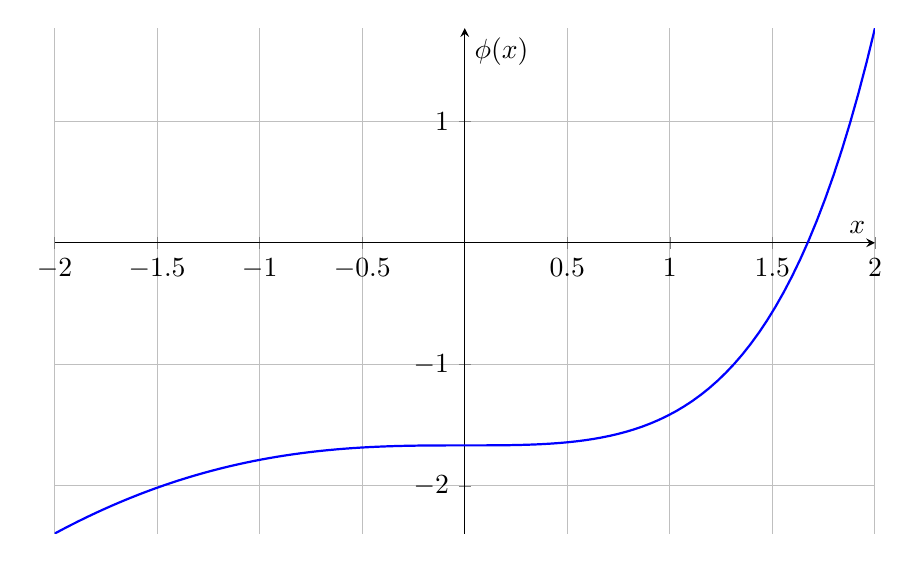
\begin{tikzpicture}
        \begin{axis}[
            axis lines = middle,
            xlabel = $x$,
            ylabel = {$\phi(x)$},
            domain=-2:2,
            samples=100,
            width=12cm,
            height=8cm,
            grid=both,
        ]
        \addplot [
            color=blue,
            thick
        ]
        { (8/27) * exp(3*x/2) - (1/3) * x^2 - (4/9) * x - 53/27 };
        \end{axis}
        \end{tikzpicture}
        \caption{Courbe représentative de $\phi(x)$.}
    \end{figure}
\end{enumerate}

\end{comment}

\section*{\underline{\textbf{\textcolor{red}{IV. Équations différentielles du 2\textsuperscript{nd} ordre à coefficients constants}}}}

Une équation différentielle du second ordre à coefficients constants est une équation de la forme :

\noindent\textbf{(E)} : $ay'' + by' + cy = g(x)$ \quad où $a, b, c \in \mathbb{R}$ avec $a \neq 0$ (Équation avec second membre).

\medskip

\noindent L'équation obtenue en remplaçant le second membre par $0$ est appelée \textbf{équation homogène} (ou équation sans second membre) associée à $(E)$ :

\noindent\textbf{(E')} : $ay'' + by' + cy = 0$ \quad où $a \neq 0$ (Équation homogène).

\subsection*{\underline{\textbf{\textcolor{red}{ Recherche de la solution homogène de (E')}}}}

Soit $(E') : ay'' + by' + cy = 0$ avec $a \neq 0$. 
Nous appelons \textbf{équation caractéristique} associée à $(E')$ l'équation du second degré : 
\textcolor{red}{$ ar^2 + br + c = 0 $}

\subsection*{\underline{\textbf{\textcolor{red}{Théorème}}}}

Soit $(E') : ay'' + by' + cy = 0$ une équation différentielle et $ar^2 + br + c = 0$ son équation caractéristique associée de discriminant $\Delta = b^2 - 4ac$.

\begin{itemize}
    \item[$\bullet$] \textbf{Si $\Delta > 0$ :} L'équation caractéristique admet deux solutions réelles distinctes :
    
    $ r_1 = \frac{-b-\sqrt{\Delta}}{2a} \quad \text{et} \quad r_2 = \frac{-b+\sqrt{\Delta}}{2a} $
    Dans ce cas, la solution générale de $(E')$ est de la forme :
    
    $ \textcolor{red}{\boxed{ y_h(x) = A e^{r_1 x} + B e^{r_2 x} }} \quad \text{où } A \text{ et } B \text{ sont des constantes réelles.} $

    \item[$\bullet$] \textbf{Si $\Delta = 0$ :} L'équation caractéristique admet une solution double réelle :
    $ r_0 = \frac{-b}{2a} $
    
    Dans ce cas, la solution générale de $(E')$ est de la forme :
    
    $ \textcolor{red}{\boxed{ y_h(x) = (Ax + B)e^{r_0 x} }} \quad \text{où } A \text{ et } B \text{ sont des constantes réelles.} $

    \item[$\bullet$] \textbf{Si $\Delta < 0$ :} L'équation caractéristique admet deux solutions complexes conjuguées :
    
    $ r_1 = \alpha + i\beta \quad \text{et} \quad r_2 = \alpha - i\beta \quad \text{avec } \alpha = \frac{-b}{2a} \text{ et } \beta = \frac{\sqrt{-\Delta}}{2a} $
    
    Dans ce cas, la solution générale de $(E')$ est de la forme :
    
    $ \textcolor{red}{\boxed{ y_h(x) = e^{\alpha x} \left( A\cos(\beta x) + B\sin(\beta x) \right) }} \quad \text{où } A \text{ et } B \text{ sont des constantes réelles.} $
\end{itemize}


\subsection*{\underline{\textbf{\textcolor{red}{Remarques}}}}
Dans tous les cas, les constantes $A$ et $B$ sont dépendantes des conditions initiales.

\subsection*{\underline{\textbf{\textcolor{red}{Exemples d'application}}}}

\textbf{Exemple 1 : Cas $\Delta > 0$} \\
Résoudre l'équation différentielle : $(E'_1) : y'' - 3y' + 2y = 0$.
\begin{itemize}
    \item L'équation caractéristique associée est : $r^2 - 3r + 2 = 0$.
    \item Calcul du discriminant : $\Delta = (-3)^2 - 4(1)(2) = 9 - 8 = 1$.
    \item Puisque $\Delta > 0$, l'équation admet deux racines réelles distinctes :
    \[ r_1 = \frac{3 - \sqrt{1}}{2(1)} = 1 \quad \text{et} \quad r_2 = \frac{3 + \sqrt{1}}{2(1)} = 2 \]
    \item La solution générale de $(E'_1)$ est donc :
    \[ \boxed{y_h(x) = A e^{x} + B e^{2x}} \quad \text{avec } A, B \in \mathbb{R} \]
\end{itemize}

\medskip

\textbf{Exemple 2 : Cas $\Delta = 0$} \\
Résoudre l'équation différentielle : $(E'_2) : y'' - 4y' + 4y = 0$.
\begin{itemize}
    \item L'équation caractéristique associée est : $r^2 - 4r + 4 = 0$.
    \item Calcul du discriminant : $\Delta = (-4)^2 - 4(1)(4) = 16 - 16 = 0$.
    \item Puisque $\Delta = 0$, l'équation admet une racine double réelle :
    \[ r_0 = \frac{4}{2(1)} = 2 \]
    \item La solution générale de $(E'_2)$ est donc :
    \[ \boxed{y_h(x) = (Ax + B)e^{2x}} \quad \text{avec } A, B \in \mathbb{R} \]
\end{itemize}

\medskip

\textbf{Exemple 3 : Cas $\Delta < 0$} \\
Résoudre l'équation différentielle : $(E'_3) : y'' - 2y' + 5y = 0$.
\begin{itemize}
    \item L'équation caractéristique associée est : $r^2 - 2r + 5 = 0$.
    \item Calcul du discriminant : $\Delta = (-2)^2 - 4(1)(5) = 4 - 20 = -16$.
    \item Puisque $\Delta < 0$, l'équation admet deux racines complexes conjuguées $r = \alpha \pm i\beta$ avec :
    \[ \alpha = \frac{-(-2)}{2(1)} = 1 \quad \text{et} \quad \beta = \frac{\sqrt{-(-16)}}{2(1)} = \frac{\sqrt{16}}{2} = 2 \]
    Les racines sont donc $r_1 = 1 + 2i$ et $r_2 = 1 - 2i$.
    \item La solution générale de $(E'_3)$ est donc :
    \[ \boxed{y_h(x) = e^{x} \left( A\cos(2x) + B\sin(2x) \right)} \quad \text{avec } A, B \in \mathbb{R} \]
\end{itemize}

\medskip

\textbf{Exemple 4 : Résolution avec conditions initiales} \\
Déterminer la solution unique de l'équation $(E'_1) : y'' - 3y' + 2y = 0$ vérifiant les conditions initiales :
\[ y(0) = 3 \quad \text{et} \quad y'(0) = 4 \]

\begin{itemize}
    \item \textbf{Étape 1 : Forme générale de la solution} \\
    D'après l'Exemple 1, la solution générale de l'équation est :
    \[ y_h(x) = A e^{x} + B e^{2x} \quad \text{avec } A, B \in \mathbb{R} \]
    
    \item \textbf{Étape 2 : Calcul de la dérivée} \\
    Pour appliquer la seconde condition, on dérive la fonction $y_h$ :
    \[ y_h'(x) = A e^{x} + 2B e^{2x} \]
    
    \item \textbf{Étape 3 : Application des conditions initiales} \\
    En injectant $x = 0$ dans les expressions de $y_h$ et $y_h'$, on obtient le système d'équations suivant :
    \[
    \begin{cases}
    y_h(0) = 3 \implies A e^{0} + B e^{0} = 3 \implies A + B = 3 \\
    y_h'(0) = 4 \implies A e^{0} + 2B e^{0} = 4 \implies A + 2B = 4
    \end{cases}
    \]
    
    \item \textbf{Étape 4 : Résolution du système} \\
    Par soustraction de la première ligne à la deuxième :
    \[ (A + 2B) - (A + B) = 4 - 3 \implies B = 1 \]
    En remplaçant $B = 1$ dans la première équation ($A + 1 = 3$), on trouve :
    \[ A = 2 \]
    
    \item \textbf{Conclusion :} \\
    La solution unique de l'équation vérifiant ces conditions initiales est :
    \[ \boxed{y(x) = 2e^{x} + e^{2x}} \]
\end{itemize}

\begin{comment}

\subsection*{\underline{\textbf{\textcolor{red}{2. Recherche d'une solution particulière de (E)}}}}

Pour trouver une solution particulière $y_p$ de l'équation complète $ay'' + by' + cy = g(x)$, on cherche une fonction $y_p$ ayant une forme similaire à celle de $g(x)$.

\begin{itemize}
    \item \textbf{Cas où $g(x)$ est un polynôme de degré $n$ :}
    \begin{itemize}
        \item Si $c \neq 0$, on cherche $y_p(x)$ sous la forme d'un polynôme de degré $n$.
        \item Si $c = 0$ et $b \neq 0$, on cherche $y_p(x)$ sous la forme $x \times P(x)$, où $P(x)$ est un polynôme de degré $n$.
        \item Si $c = 0$ et $b = 0$, on cherche $y_p(x)$ sous la forme $x^2 \times P(x)$.
    \end{itemize}

    \item \textbf{Cas où $g(x) = P(x)e^{\mu x}$ (avec $P$ un polynôme de degré $n$) :}
    \begin{itemize}
        \item Si $\mu$ n'est pas racine de l'équation caractéristique, on cherche : \\ $y_p(x) = Q(x)e^{\mu x}$ avec $\deg(Q) = \deg(P)$.
        \item Si $\mu$ est racine simple de l'équation caractéristique, on cherche : \\ $y_p(x) = x \cdot Q(x)e^{\mu x}$.
        \item Si $\mu$ est racine double de l'équation caractéristique, on cherche : \\ $y_p(x) = x^2 \cdot Q(x)e^{\mu x}$.
    \end{itemize}

    \item \textbf{Cas où $g(x) = \alpha \cos(\omega x) + \mu \sin(\omega x)$ :}
    \begin{itemize}
        \item Si $i\omega$ n'est pas racine de l'équation caractéristique, on cherche $y_p$ sous la forme :
        \[ y_p(x) = A \cos(\omega x) + B \sin(\omega x) \]
        \item Si $i\omega$ est racine de l'équation caractéristique (ce qui arrive si $b=0$ et $\omega = \sqrt{c/a}$), on cherche $y_p$ sous la forme :
        \[ y_p(x) = x \left( A \cos(\omega x) + B \sin(\omega x) \right) \]
    \end{itemize}
\end{itemize}

\noindent\textbf{Exemple (Cas sans résonance) :} 
Trouver une solution particulière de $(E) : y'' - 3y' + 2y = 2x^2 + 1$.

\textbf{Solution :} 
Le second membre est un polynôme de degré 2 et le coefficient $c = 2 \neq 0$. On cherche donc $y_p$ sous la forme $y_p(x) = Ax^2 + Bx + C$.
On calcule les dérivées :
\[ y_p'(x) = 2Ax + B \quad \text{et} \quad y_p''(x) = 2A \]
En injectant dans $(E)$ :
\[ (2A) - 3(2Ax + B) + 2(Ax^2 + Bx + C) = 2x^2 + 1 \]
\[ 2Ax^2 + (-6A + 2B)x + (2A - 3B + 2C) = 2x^2 + 1 \]
Par identification :
\[
\begin{cases}
2A = 2 \implies A = 1 \\
-6A + 2B = 0 \implies 2B = 6 \implies B = 3 \\
2A - 3B + 2C = 1 \implies 2(1) - 3(3) + 2C = 1 \implies 2C = 8 \implies C = 4
\end{cases}
\]
La solution particulière est donc : $\boxed{y_p(x) = x^2 + 3x + 4}$.

\subsection*{\underline{\textbf{\textcolor{red}{3. Solution générale de (E)}}}}
Soit $f_{2}(x)$ solution générale de \textbf{(E')}, si $f_{1}(x)$ donnée, est solution particulière de \textbf{(E)}, alors la solution générale de \textbf{(E)}; $y(x)$,sera de la forme \[y(x)=f_{2}(x)+f_{1}(x) \]
\subsection*{\underline{\textbf{\textcolor{red}{Exemple}}}}
Résoudre l'équation différentielle \textbf{(E:)}$y''-4y'+3y=0$ puis, déterminer et représenter graphiquement la solution qui passe par l'origine $O(0,0)$ du repère et dont la dérivée vaut 1 en 0.
\subsection*{\underline{\textbf{\textcolor{green}{Solution}}}}
\subsection*{\underline{\textbf{\textcolor{green}{1. Résolution de l'équation différentielle homogène}}}}
L'équation différentielle donnée est une équation linéaire homogène d'ordre 2 à coefficients constants :
\[
y'' - 4y' + 3y = 0
\]
Pour résoudre cette équation, nous cherchons les racines de l'équation caractéristique associée :
\[
r^2 - 4r + 3 = 0
\]
Cette équation se factorise facilement :
\[
(r - 3)(r - 1) = 0
\]
Les racines sont :
\[
r_1 = 3 \quad \text{et} \quad r_2 = 1
\]
Ainsi, la solution générale de l'équation différentielle est :
\[
y(x) = C_1 e^{3x} + C_2 e^x
\]

\subsection*{\underline{\textbf{\textcolor{green}{2. Détermination de la solution particulière}}}}
Nous devons maintenant déterminer les constantes $C_1$ et $C_2$ en utilisant les conditions initiales données :
\[
y(0) = 0 \quad \text{et} \quad y'(0) = 1
\]
Calculons $y'(x)$ à partir de la solution générale :
\[
y'(x) = 3C_1 e^{3x} + C_2 e^x
\]
En utilisant les conditions initiales :
\[
y(0) = C_1 e^0 + C_2 e^0 = C_1 + C_2 = 0 \quad \Rightarrow \quad C_2 = -C_1
\]
\[
y'(0) = 3C_1 e^0 + C_2 e^0 = 3C_1 + C_2 = 1
\]
Substituons $C_2 = -C_1$ dans la deuxième équation :
\[
3C_1 - C_1 = 1 \quad \Rightarrow \quad 2C_1 = 1 \quad \Rightarrow \quad C_1 = \frac{1}{2}
\]
\[
C_2 = -\frac{1}{2}
\]
La solution particulière est donc :
\[
y(x) = \frac{1}{2} e^{3x} - \frac{1}{2} e^x
\]

\subsection*{\underline{\textbf{\textcolor{green}{3. Représentation graphique}}}}

Pour représenter graphiquement la solution $y(x) = \frac{1}{2} e^{3x} - \frac{1}{2} e^x$, nous traçons la courbe dans un repère.

\begin{figure}[h!]
    \centering
    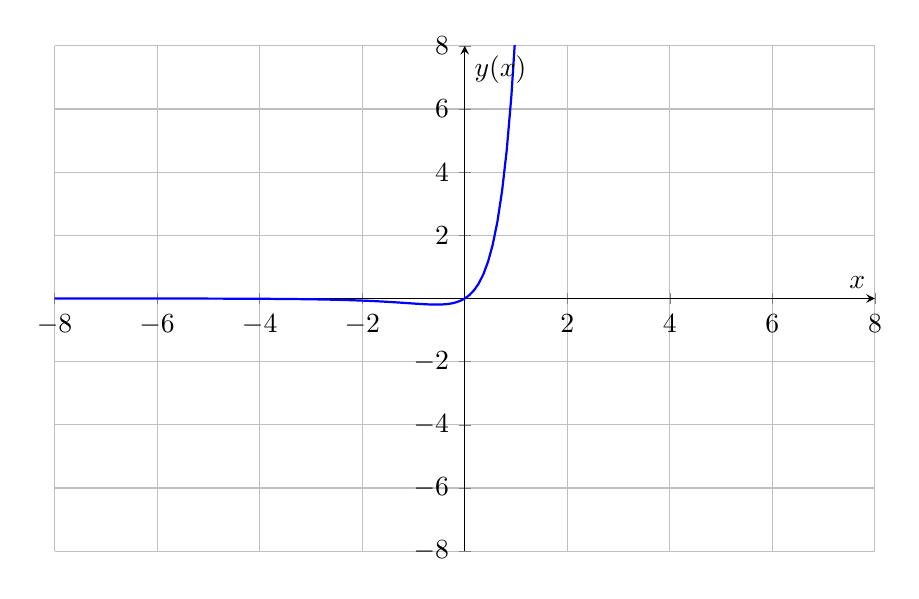
\begin{tikzpicture}
    \begin{axis}[
        axis lines = middle,
        xlabel = $x$,
        ylabel = {$y(x)$},
        domain=-8:1,
        xmin=-8, xmax=8,
        ymin=-8, ymax=8,
        samples=100,
        width=12cm,
        height=8cm,
        grid=both,
    ]
    \addplot [
        color=blue,
        thick
    ]
    { (1/2) * exp(3*x) - (1/2) * exp(x) };
    \end{axis}
    \end{tikzpicture}
    \caption{Courbe représentative de $y(x) = \frac{1}{2} e^{3x} - \frac{1}{2} e^x$.}
\end{figure}
\end{comment}
\end{document}
